\documentclass[a4paper]{article}

\usepackage[english]{babel}
\usepackage[utf8]{inputenc}
\usepackage{amsmath}
\usepackage{graphicx}
\usepackage[colorinlistoftodos]{todonotes}

\title{Final Year Project Progress Report}

\author{Samuel Lee}

\date{16 January 2019}

\begin{document}
\maketitle

\begin{abstract}
The given data is sales data of 66 products sold over a period of 11 days without any changes in price and under some sales promotion. The objective is to use Thompson sampling to increase sales revenue in the long run and also investigate if different approaches of Thompson sampling will yield different results.
\end{abstract}

\section{Understanding the data}
\label{sec:introduction}
\begin{figure}
\centering
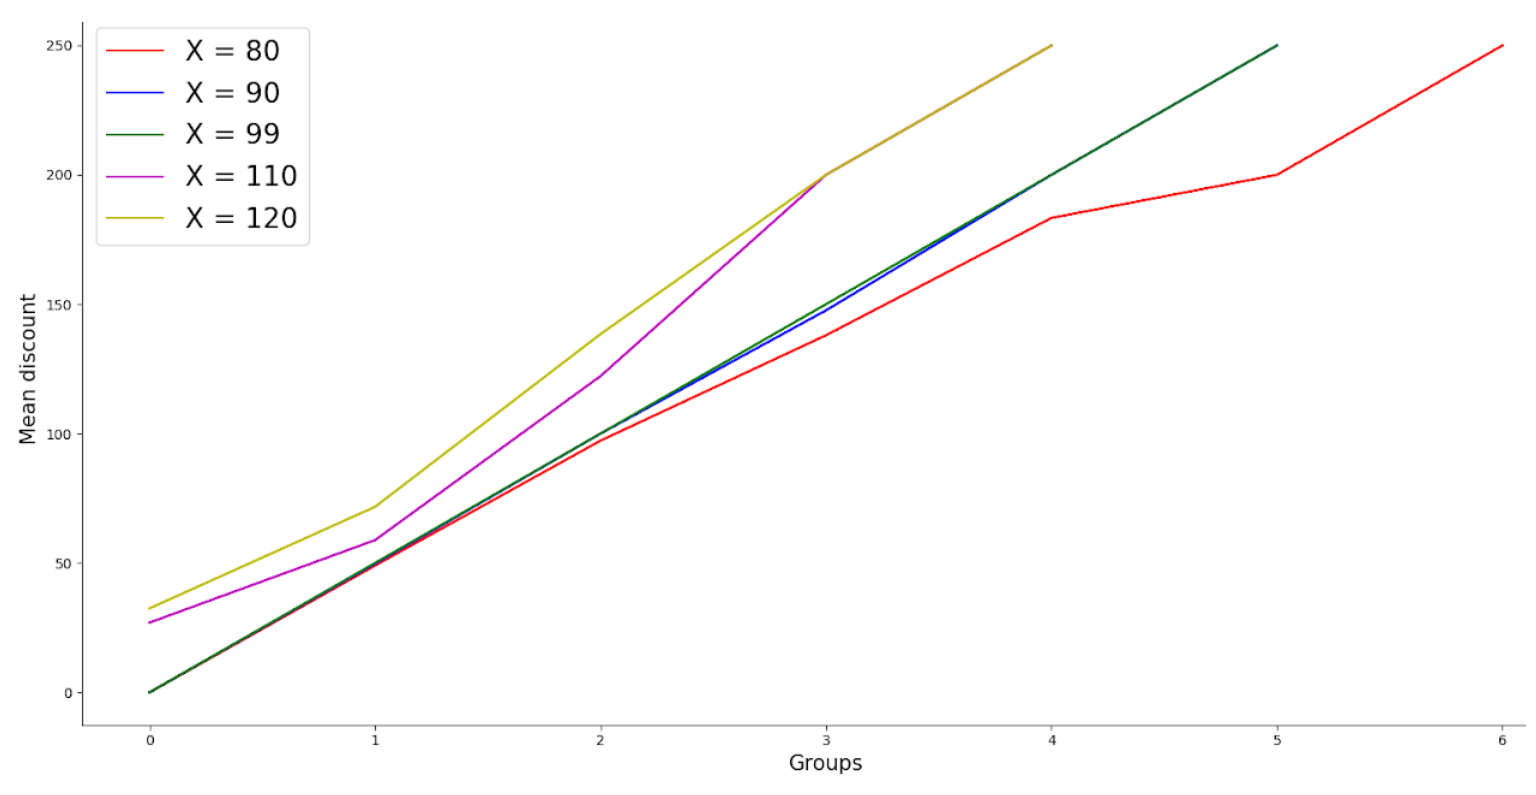
\includegraphics[width=1\textwidth]{cut.png}
\caption{\label{fig:cut}Plotting mean discounts for each group.}
\end{figure}

It is known that there is an ongoing sales promotion in the data in which an order would be eligible for discounts by fulfilling a minimum value. This value is defined as the threshold. For example, every \$99 spent would be eligible for a \$50 discount. One possible method to find the threshold would be through trial and error.
\newline
\newline
If $X$ is trialed as the threshold value, orders can be categorized into groups of different multiples of $X$. The first group would consist of orders ranging from \$0 to \$($X$-1) and the second group would range from \$$X$ to \$2$X$-1 and so on. The mean discount for each group can then be calculated. If $X$ is the threshold value, the mean discount for the first group should be 0 as all orders in that group should not have fulfilled the minimum amount. Likewise, the mean discount for subsequent groups should be multiples of the discount. Plotting the mean discounts for each group should reveal a linear relationship.
\newline
\newline
For this data set, multiple values of $X$ (80, 90, 99, 110, 120) were tested and the mean discounts were plotted. For $X = 80, 110$ and $120$, the gradients are not constant over each group. This suggests that some groups contain orders that qualify for different discounts from the rest. The plots of $X = 90$ and $X = 99$ indicate a strong linear relationship. However, at $Groups = 3$, the plot of $X = 90$ is not as linear as $X=99$. Thus, it is likely that the true threshold value of this data set is 99.

\section{Description of approaches}
\label{sec:approach}
The first approach would be to use the classical Thompson sampling algorithm in a multi-armed bandit problem where each price vector represents an arm and the objective is to investigate which arm has the highest expected payout so as to maximize revenue over time. In this approach, there is a finite number of price vectors and the goal is to learn the demand distribution of each price vector.
\newline
\newline
The second approach would be to use Thompson sampling in a dynamic pricing algorithm. In this approach, there is usually a larger set (possibly infinite) of price vectors. In this approach, the goal is to learn the distribution of the price elasticity of each product and not the distribution under each price vector.

\section{Generating training data}
\label{sec:theory}
Since the data set only contained sales data for one set of prices, there is insufficient data to perform Thompson sampling. Thus, simulation data was created and the set of prices in the data set was used as one price vector. 
\newline
\newline
For each price vector $i$, a theoretical sales data was created using the formula below and it represents the true demand under this price vector.
\[X_i = \frac{e^{V_i - P_i}}{\sum_{j=0}^{N}e^{V_j - P_j}}\]
where $V_i$ represents the customer's valuation of product $i$ and $P_i$ is the price of product $i$. In the denominator, $j=0$ represents the option where the customer chooses not to buy anything. For the first approach, in addition to the original price vector, two other price vectors were created where the first vector is created by adding 5 to the original price vector and the second vector is created by subtracting 5 from the original price vector. 
\newline
\newline
As there are now 3 price vectors, the valuation vector $V$ can be created by randomly sampling from a 5\% neighbourhood of $\hat{P}$ where $\hat{P}=\sum_{k=1}^{3}P_k$. $V_0$ is randomly sampled from the interval $(0,5).$
\newline
\newline
With the $V$ and $P$ vectors defined, the theoretical $X_i$ corresponding to each price vector can be created and they will represent the true demand. In the long run, the expected value of all data points for each price vector should be equal to the theoretical $X_i$.
\newline
\newline
For each price vector, 20 data points were created. In order to ensure that the expected value of all data points was equal to the theoretical $X_i$, 10 epsilon vectors were created and the data points were obtained by adding and subtracting the epsilon vector from the theoretical $X_i$. This process was repeated for the other two price vectors as well. In total, there were 60 data points created with each price vector having 20 data points.

\section{First approach}
In this approach, it is assumed that the true demand function under each price vector follows a normal distribution. The prior distribution was then estimated from the 20 data points generated earlier using maximum likelihood estimation. 

\section{Results and interpretation 2-3 pages}
Show a graph of the longitudinal resistivity ($\rho_{xx}$) and Hall resistivity ($\rho_{xy}$) versus magnetic field, extracted from the raw data shown in figure \ref{fig:data}. You will have the link to the data in your absalon messages, if not e-mail Guen (guen@nbi.dk). Explain how you calculated these values, and refer to the theory.


\subsection{Classical regime}
Calculate the sheet electron density $n_{s}$ and electron mobility $\mu$ from the data in the low-field regime, and refer to the theory in section \ref{sec:theory}. Explain how you retrieved the values from the data (did you use a linear fit?).
Round values off to 1 or 2 significant digits: 8.1643 ~= 8.2. Also, 5e-6 is easier to read than 0.000005.

!OBS: This part is optional (only if you have time left).
Calculate the uncertainty as follows: \newline $u(f(x, y, z)) = \sqrt{(\frac{\delta f}{\delta{x}} u(x))^{2} + (\frac{\delta f}{\delta{y}} u(y))^{2} + (\frac{\delta f}{\delta{z}} u(z))^{2}}$, where $f$ is the calculated value ($n_{s}$ or $\mu$), $x, y, z$ are the variables taken from the measurement and $u(x)$ is the uncertainty in x (and so on).

\subsection{Quantum regime}
Calculate $n_{s}$ for the high-field regime.
Show a graph of the longitudinal conductivity ($\rho_{xx}$) and Hall conductivity($\rho_{xy}$) \textbf{in units of the resistance quantum} ($\frac{h}{e^{2}}$), depicting the integer filling factors for each plateau.
Show a graph of the plateau number versus its corresponding value of $1/B$. From this you can determine the slope, which you use to calculate the electron density.
Again, calculate the uncertainty for your obtained values.

\section{Discussion 1/2-1 page}
Discuss your results. Compare the two values of $n_{s}$ that you've found in the previous section. Compare your results with literature and comment on the difference. If you didn't know the value of the resistance quantum, would you be able to deduce it from your measurements? If yes/no, why?

\newpage
\section{Some LaTeX tips}
\label{sec:latex}
\subsection{How to Include Figures}

First you have to upload the image file (JPEG, PNG or PDF) from your computer to writeLaTeX using the upload link the project menu. Then use the includegraphics command to include it in your document. Use the figure environment and the caption command to add a number and a caption to your figure. See the code for Figure \ref{fig:frog} in this section for an example.

\begin{figure}
\centering
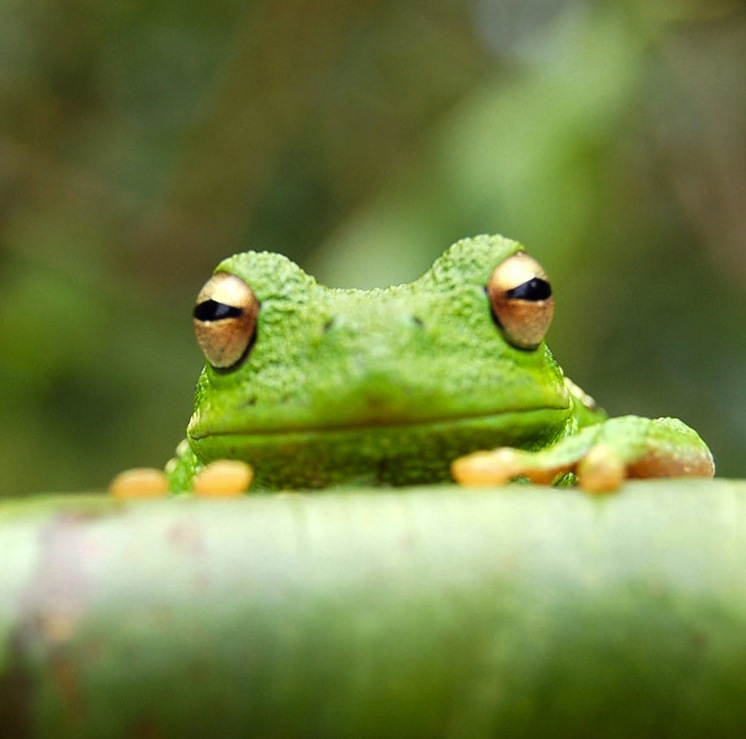
\includegraphics[width=0.3\textwidth]{frog.jpg}
\caption{\label{fig:frog}This frog was uploaded to writeLaTeX via the project menu.}
\end{figure}

\subsection{How to Make Tables}

Use the table and tabular commands for basic tables --- see Table~\ref{tab:widgets}, for example.

\begin{table}
\centering
\begin{tabular}{l|r}
Item & Quantity \\\hline
Widgets & 42 \\
Gadgets & 13
\end{tabular}
\caption{\label{tab:widgets}An example table.}
\end{table}

\subsection{How to Write Mathematics}

\LaTeX{} is great at typesetting mathematics. Let $X_1, X_2, \ldots, X_n$ be a sequence of independent and identically distributed random variables with $\text{E}[X_i] = \mu$ and $\text{Var}[X_i] = \sigma^2 < \infty$, and let

\begin{equation}
S_n = \frac{X_1 + X_2 + \cdots + X_n}{n}
      = \frac{1}{n}\sum_{i}^{n} X_i
\label{eq:sn}
\end{equation}

denote their mean. Then as $n$ approaches infinity, the random variables $\sqrt{n}(S_n - \mu)$ converge in distribution to a normal $\mathcal{N}(0, \sigma^2)$.

The equation \ref{eq:sn} is very nice.

\subsection{How to Make Sections and Subsections}

Use section and subsection commands to organize your document. \LaTeX{} handles all the formatting and numbering automatically. Use ref and label commands for cross-references.

\subsection{How to Make Lists}

You can make lists with automatic numbering \dots

\begin{enumerate}
\item Like this,
\item and like this.
\end{enumerate}
\dots or bullet points \dots
\begin{itemize}
\item Like this,
\item and like this.
\end{itemize}
\dots or with words and descriptions \dots
\begin{description}
\item[Word] Definition
\item[Concept] Explanation
\item[Idea] Text
\end{description}

We hope you find write\LaTeX\ useful, and please let us know if you have any feedback using the help menu above.

\begin{thebibliography}{9}
\bibitem{nano3}
  K. Grove-Rasmussen og Jesper Nygård,
  \emph{Kvantefænomener i Nanosystemer}.
  Niels Bohr Institute \& Nano-Science Center, Københavns Universitet

\end{thebibliography}
\end{document}